\documentclass{webofc}
\usepackage[varg]{txfonts}
% review
%\usepackage[textwidth=120]{todonotes}
%\usepackage{color}
\usepackage{subcaption}

\begin{document}
\title{About some question in modern models of thunderstorm runway breakdown}
\author{\firstname{Mikhail} \lastname{Zelenyi}\inst{1,2,3}\fnsep\thanks{\email{mihail.zelenyy@phystech.edu}} \and
    \firstname{Egor} \lastname{Stadnichuk}\inst{1,2} \and \firstname{Alexander} \lastname{Nozik}\inst{1,2}\fnsep\thanks{\email{altavir@gmail.com}}  
    }
%
\institute{Institute for Nuclear Research of RAS
    \and
    Moscow Institute of Physics and Technology (State University) 
    \and
    Space Research Institute of RAS
}
\abstract{%
    In modern models based on runway breakdown and created for explaining initiation of lighting and TGF phenomenon, there has been a strong emphasis on peak of positron annihilation in observed gamma-ray spectra. This observation used as evidence importance of positron feedback in thunderstorms. But in this report, we give some result of Monte-Carlo simulations speaking about weak influence of positrons on thunderstorm processes and appearance of TGF.
}
%
\maketitle

\section{Introduction}
Despite decades of investigations and observations, there are gaps in physics of atmospheric discharge. Nowadays it is widely known how lightning is created under thundercloud conditions. However, the mechanism of cloud ionization is not described accurately. Either various revealing effects appearing in thunderstorms were not precisely described. For example, in strong correlation with thunderstorms TGFs are observed. TGF or terrestrial gamma ray flashes – enormous bursts of gamma-ray radiation detected from thunderclouds. This phenomenon has several explanations but none of them is considered satisfying.
\begin{figure}[ht!]
	\begin{subfigure}[b]{0.5\textwidth}
    	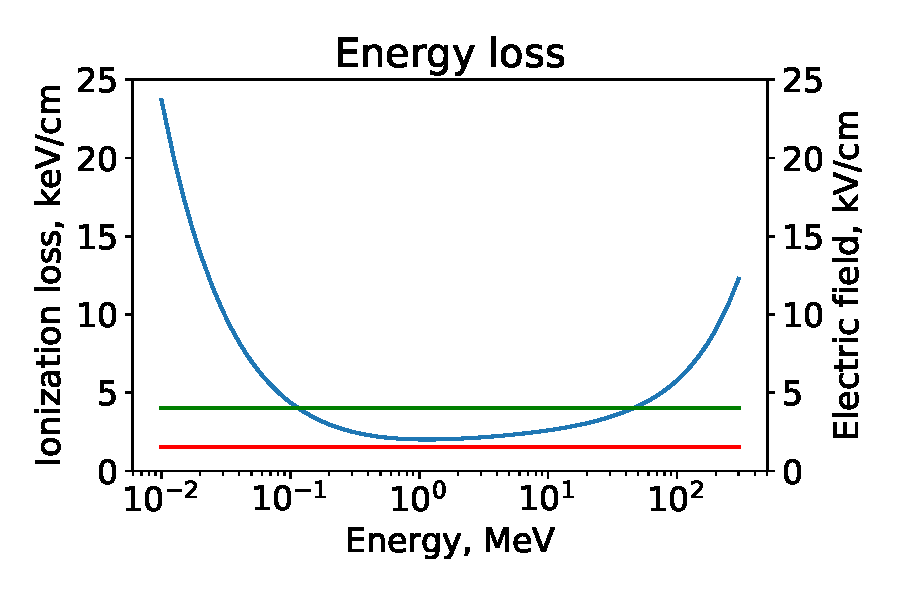
\includegraphics[width=0.95\linewidth]{pictures/01_Gurevich}
        \caption{}
        \label{pic-02-a}
    \end{subfigure}
	~
    \begin{subfigure}[b]{0.5\textwidth}
		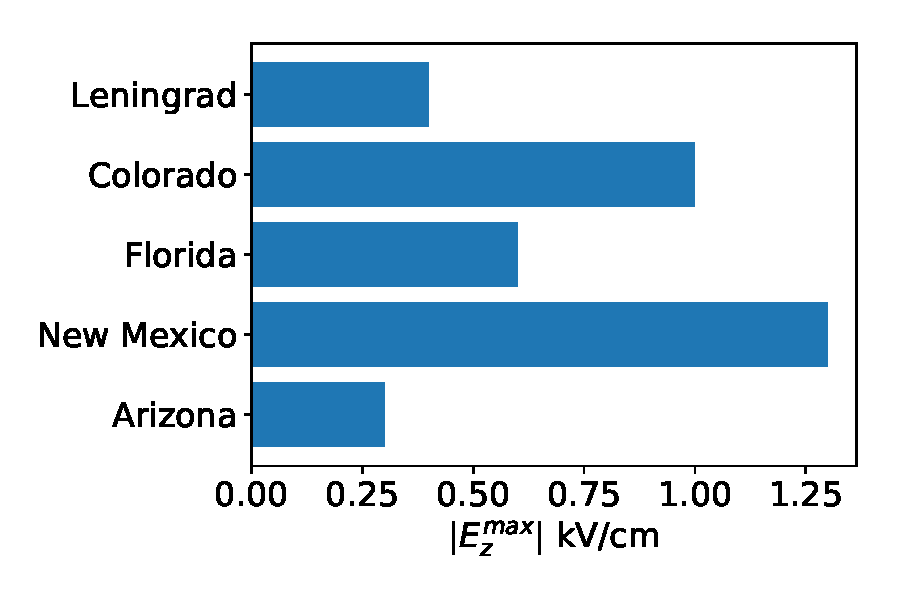
\includegraphics[width=0.95\textwidth]{pictures/03_extremal_field}
        \caption{}
        \label{pic-02-b}
    \end{subfigure}
    \caption{
    a) Gurevich model: if electric field higher than MIP loss (green line) that possibly generation runway electron, otherwise (red line) avalanches discharged.
%     a) Distribution of horizontal electric field ~\cite{mazin1989clouds} 
    b) Extremal value of vertical electric field (before 1989 y.)~\cite{mazin1989clouds}}
\end{figure}

Gurevich has made a notable contribution in understanding of electron avalanche physics in atmosphere~\cite{gurevich1992runaway}. According to his research, cosmic ray shower particles accelerate in thundercloud electric field with intensive ionization. Gurevich studied electron behavior in air with electric field. Energetic electrons that are able to accelerate under such conditions are named runaway electrons. In the following works, Gurevich developed the runaway theory~\cite{gurevich1999lightning,gurevich2001kinetic}. Nevertheless, the flux of cosmic ray showers is not intensive enough to explain cloud charging with only runaway electron ionization.
Dwyer proposed a mechanism of positron feedback that increases the runaway electron flux ~\cite{dwyer2003fundamental}. Dwyer investigated his model in the cell with electric field value 1000 kilovolt per meter. A cell is a cylinder of air with electric field. Dwyer’s feedback mechanism is described briefly as follows. A runaway electron propagating through such a cell radiates bremsstrahlung. If the bremsstrahlung photon has enough energy, then it can produce an electron-positron pair. The positron charge is opposite to the electron charge. That is why positron reverses in electric field and then propagates in direction opposite to the runaway electron motion direction. Such positrons produce ionized electrons at the beginning of primary runaway electron track. Then ionization electrons can reverse in the electric field and propagate through cell creating secondary electron avalanche. The runaway theory with Dwyer feedback mechanism is considered as one of the most reliable theory describing processes appearing in thunderclouds before lightning strike.


Experimentally observed thundercloud electric field is less than 200 kilovolts per meter (see pic.~\ref{pic-02-b} and ~\cite{}).However, there are no results the in literature regarding how positron feedback works under such conditions. The aim of the present work is to reveal whether Dwyer model operates in cells with uniform electric field less than 200 kilovolts per meter and air density between 0.3 and 0.8 kilogram per cubic meter and to calculate positron feedback coefficients for different electric fields. The algorithm of feedback coefficient calculating is described in methodology section.
The results of the investigation are negative. The paper shows that positron feedback coefficient is much less than 1 in cells with electric field under 200 kilovolts per meter. That means that one electron avalanche does not create secondary avalanches by positron feedback mechanism. The accurate value of positron feedback coefficient is stated in results section.

\section{Methodology}
Aim of our research is estimate of coefficient of reproduction (gain) for gamma and positron feedback. We define gain coefficient for gamma (positron) feedback as number of secondary particles born by gamma (positron) feedback to number of primary electron  ratio. For this we conduct simulation using Geant4 transport code~\cite{ALLISON2016186}. For improvement of performance we split our simulation on two parts:
\begin{itemize}
\item Firstly, we compute spectra of positrons and gamma-rays in avalanche for different energies of primary electron and select only those positrons and gamma-rays that could produce secondary avalanches;
\item Secondly, we compute spectrum of secondary electron created by positrons and gamma-rays and select those electron that could produce new avalanches.
\end{itemize}
As rule for validation of particle we use two condition:
\begin{itemize}
\item Particle energy is higher than runway energy.
\item Positron (electron) energy and angle should allow it to be reversed in electric field without stopping.
\end{itemize}
Then gain coefficient describable next formula:
\begin{equation}
\label{eq-gain}
\gamma_{e^+, \gamma} = \int N_{e^+, \gamma}(E_{pr},P_{e^+, \gamma}) 
N_{e^-}(P_{e^+, \gamma}, P_{e^-})
I[E_{e^+, \gamma}, E_{e^-} > E_{rw}] I[\theta_{e^-, e^+} > \theta_{c}]
~dE_{pr}~dP_{e^+, \gamma}~dP_{e^-},
\end{equation}
where $N_{e^+, \gamma}$ --- number of positrons (gamma-quanta) with four-momentum $P_{e^+, \gamma}$ per primary electron with energy $E_{pr}$, $N_{e^-}$ --- number new primary electron with four-momentum $P_{e^-}$ per positron (gamma-quantum), $E_{rw}$ --- energy of runway, $\theta_{e^-, e^+}$ --- angle between particle and electric field directions, $\theta_c$ --- critical angle of reversal in electric field,   $I[condition]$ is $1$ if condition is true and $0$ otherwise.
\section{Simulations and Results}

\begin{figure}[ht!]
	\begin{subfigure}[b]{0.5\textwidth}
    	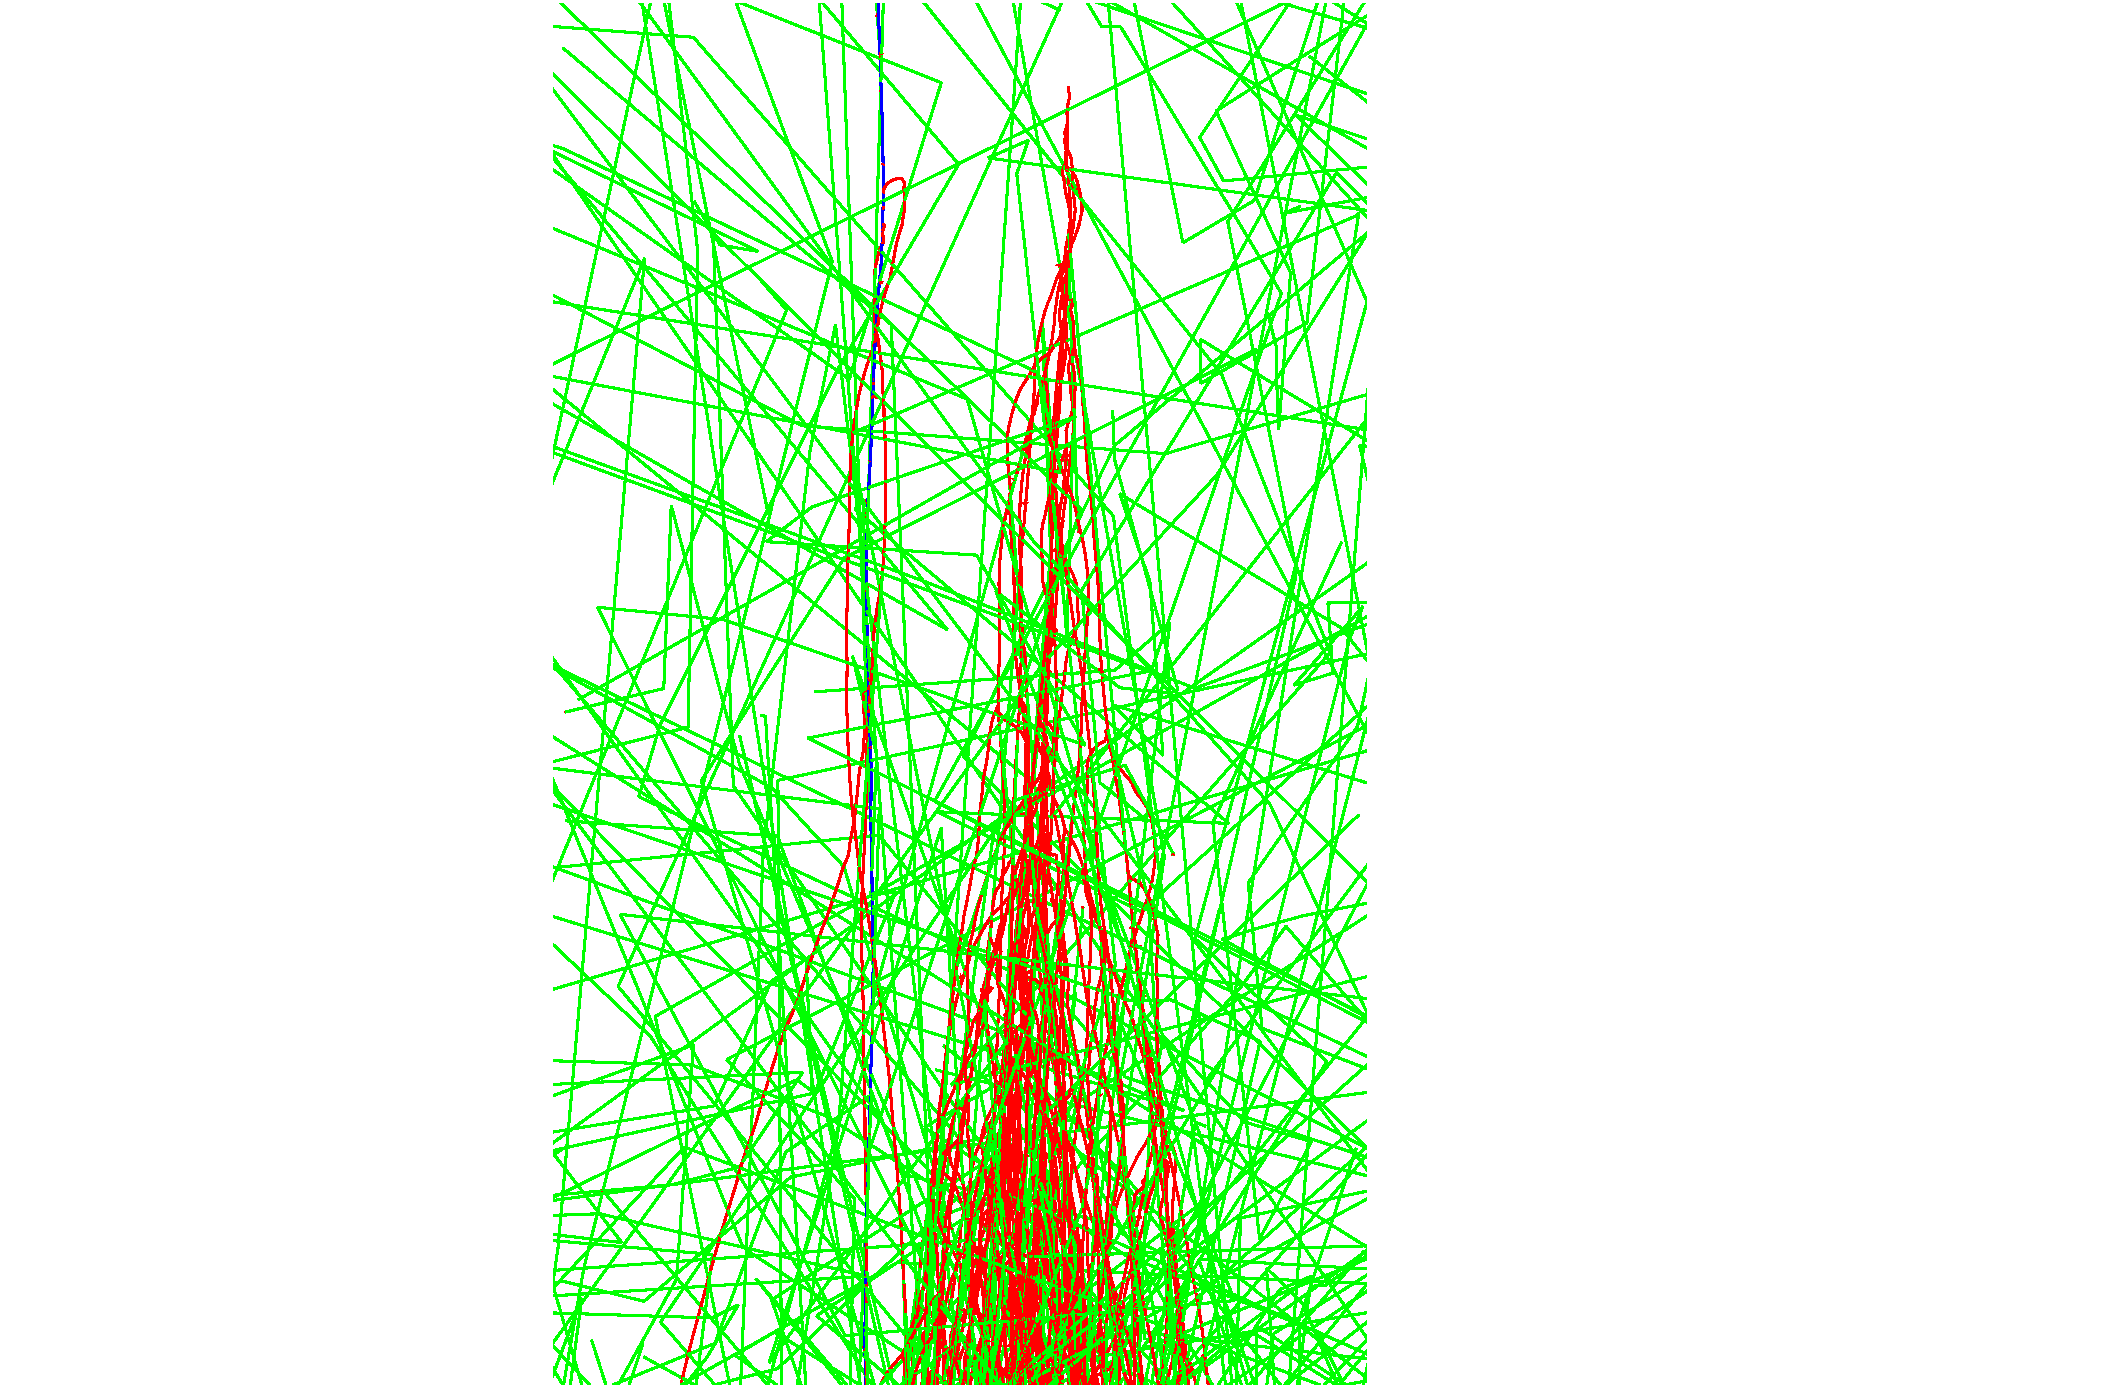
\includegraphics[width=0.95\linewidth]{pictures/10_dwyer}
        \caption{}
        \label{pic-dwyer-a}
    \end{subfigure}
	~
    \begin{subfigure}
        \begin{subfigure}[b]{0.22\textwidth}
		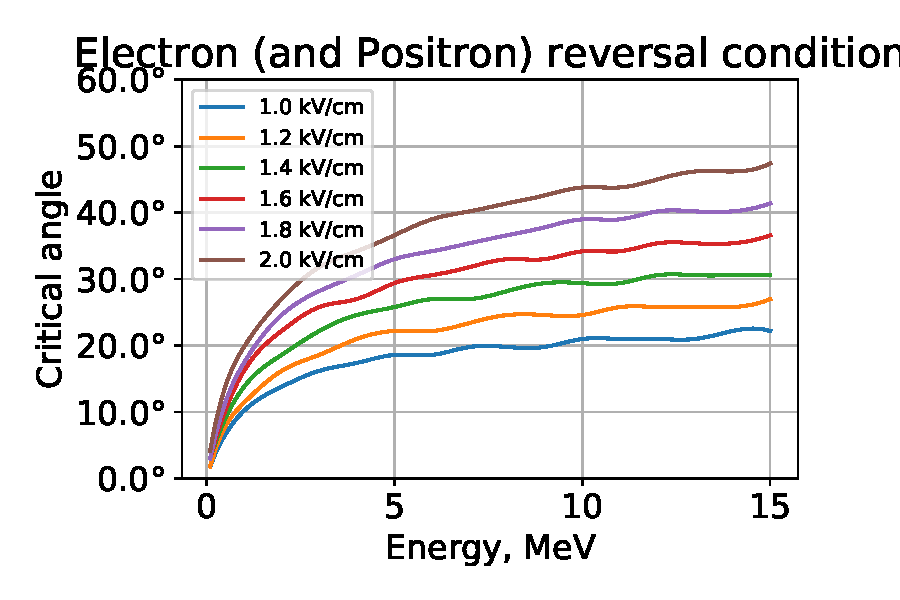
\includegraphics[width=0.95\textwidth]{pictures/09_condition}
        \caption{}
        \label{pic-reverse-b}
    \end{subfigure}
    ~
      \begin{subfigure}[b]{0.22\textwidth}
		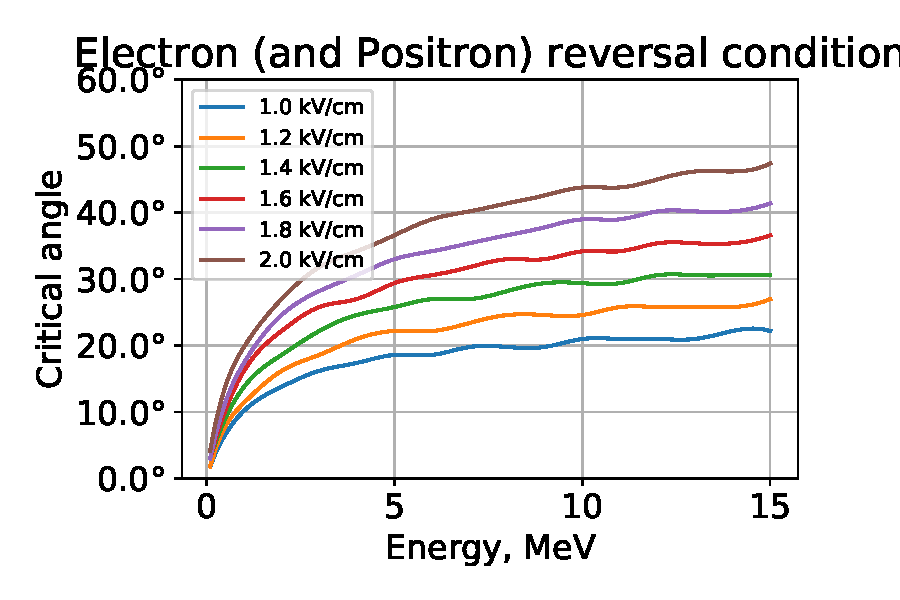
\includegraphics[width=0.95\textwidth]{pictures/09_condition}
        \caption{}
        \label{pic-reverse-b}
    \end{subfigure}
    \end{subfigure}

    \caption{
%     a) Gurevich model: if electric field higher than MIP loss (green line) that possibly generation runway electron, otherwise (red line) avalanches discharged. 
    a) Dwyer model in Geant 4 simulation. Red tracks – electrons. Blue tracks – positrons. Green tracks - gamma-rays
    b) Minimum reversal angle between electron motion direction in moment of its birth and electric field depending on electron energy. All of electrons situated above the curve are able to generate secondary electron avalanche in the cell. According to this graph, less than 50\% of electrons produced by positrons will generate secondary electron flux}
\end{figure}

We conduct simulation in accordance with methodology. In first, we compute selection condition. Minimal particle energy is determined from value of electric field and ionization loss curve (~\ref{pic-01-a}). Particles ability to turn in electric field is calculate in dry friction model, mean ionization loss involved as friction force, bremsstrahlung were not taken into account due to their smallness compared with ionization losses. From this model, for every energy, we get critical angle between field and particle momentum direction, at which particles couldn't to reverse in field. As example on pic. ~\ref{pic-01-b} draw critical angle for cloud at height 8 km.

\begin{figure}[ht!]
	\begin{subfigure}[b]{0.5\textwidth}
    	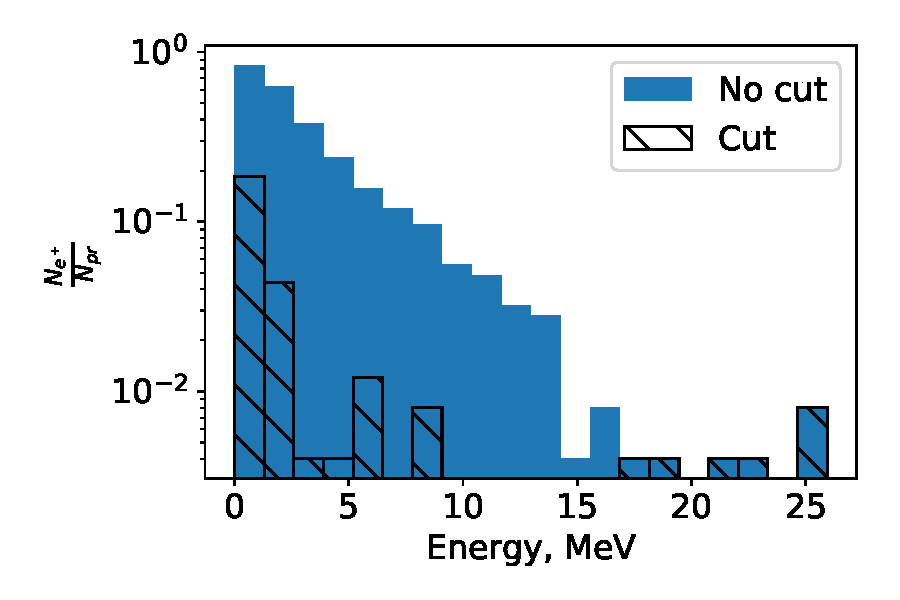
\includegraphics[width=0.95\linewidth]{pictures/04_energy_cut_positron}
        \caption{}
        \label{pic-positron-cut-a}
    \end{subfigure}
	~
    \begin{subfigure}[b]{0.5\textwidth}
		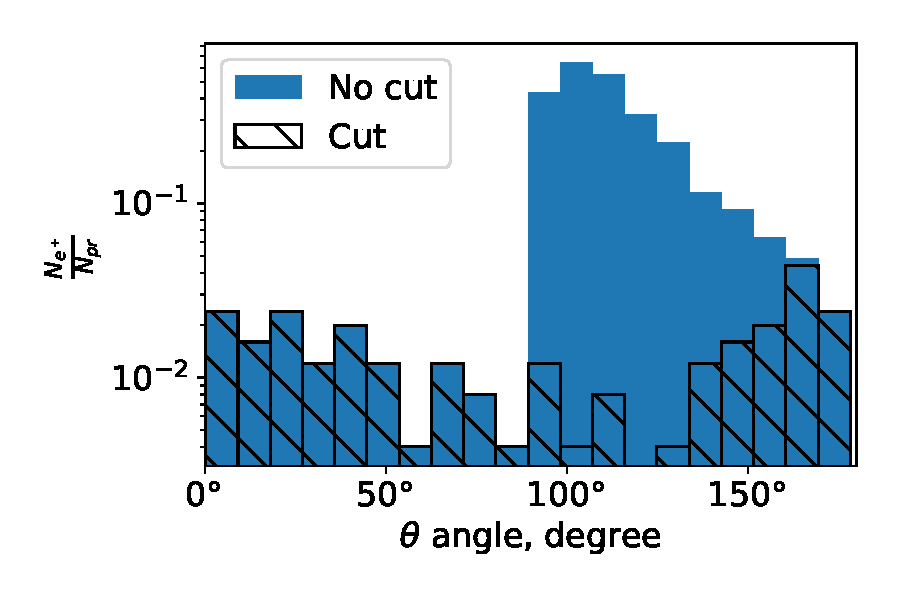
\includegraphics[width=0.95\textwidth]{pictures/05_theta_cut_positron}
        \caption{}
        \label{pic-positron-cut-b}
    \end{subfigure}
    \caption{ a) Energy b) polar angle positron distribution after and before cut for next parameters: primary electron energy - 1 MeV, field area size - 400 meter, electric field 2.5 kV/cm, air density - $0.5 kg/m^3$ ($\sim 0.5 atm$)}
\end{figure}

Further, we calculate positron, gamma and thirdly electron spectra. In simulation we consider cylindric area with different parameters set: electric field under $2.5 kV/cm$, air density between $0.3$ and $0.8 kg/m^3$ (clouds height from 4 to 12 km), field area size  200-400 meters, primary electron energy between 1 and 10 MeV.

\begin{figure}[ht!]
	\begin{subfigure}[b]{0.5\textwidth}
    	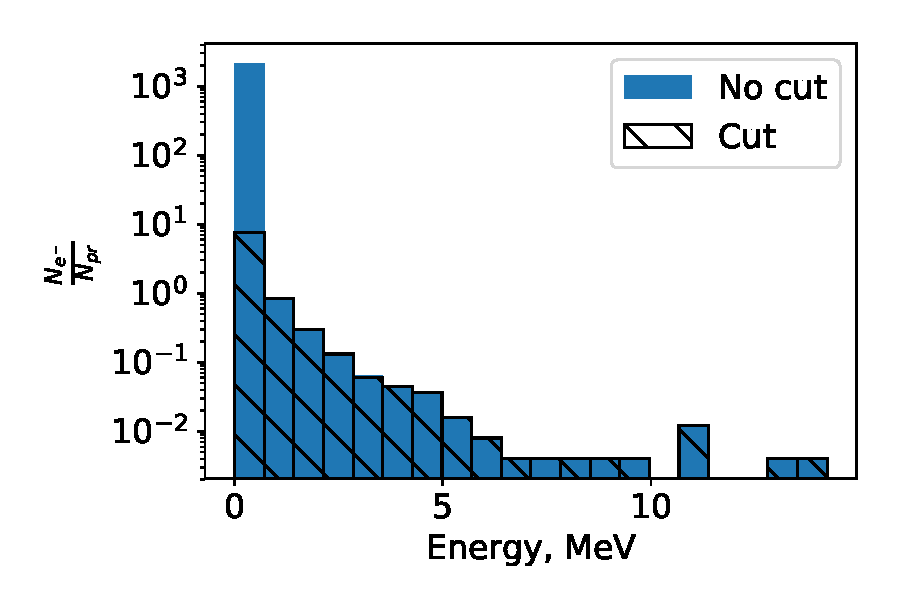
\includegraphics[width=0.95\linewidth]{pictures/06_energy_cut_electron}
        \caption{}
        \label{pic-electron-cut-a}
    \end{subfigure}
	~
    \begin{subfigure}[b]{0.5\textwidth}
		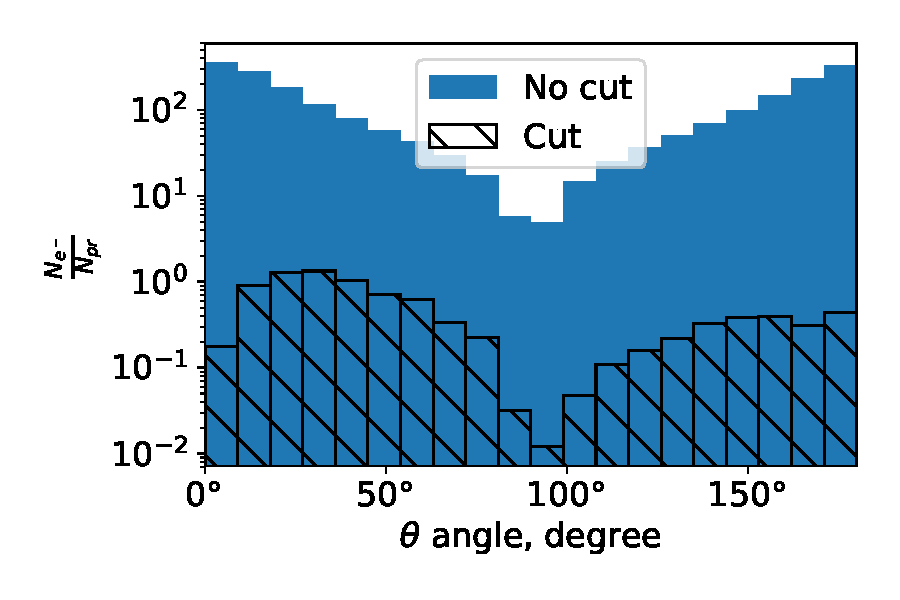
\includegraphics[width=0.95\textwidth]{pictures/07_theta_cut_electron}
        \caption{}
        \label{pic-electron-cut-b}
    \end{subfigure}
    \caption{ a) Energy b) polar angle thirdly electron distribution after and before cut for next parameters: primary electron energy - 1 MeV, field area size - 400 meter, electric field 1.5 kV/cm, air density - $0.3 kg/m^3$ ($\sim 0.2 atm$)}
\end{figure}

As example we present some spectra. On pic.~\ref{pic-positron-cut-a} and pic.~\ref{pic-positron-cut-b} draw spectrum of positron after and before involving selection rules. Analogy spectrum in another simulation parameters for third electrons shown on pic.~\ref{pic-electron-cut-a} and pic.~\ref{pic-electron-cut-b}

Using simulation result we calculate gain coefficient by formula~\ref{eq-gain} and its is small. As example gain coefficient for parameters on pic.~\ref{pic-gain-a} is less 0.01.
\begin{figure}[ht!]
\begin{center}
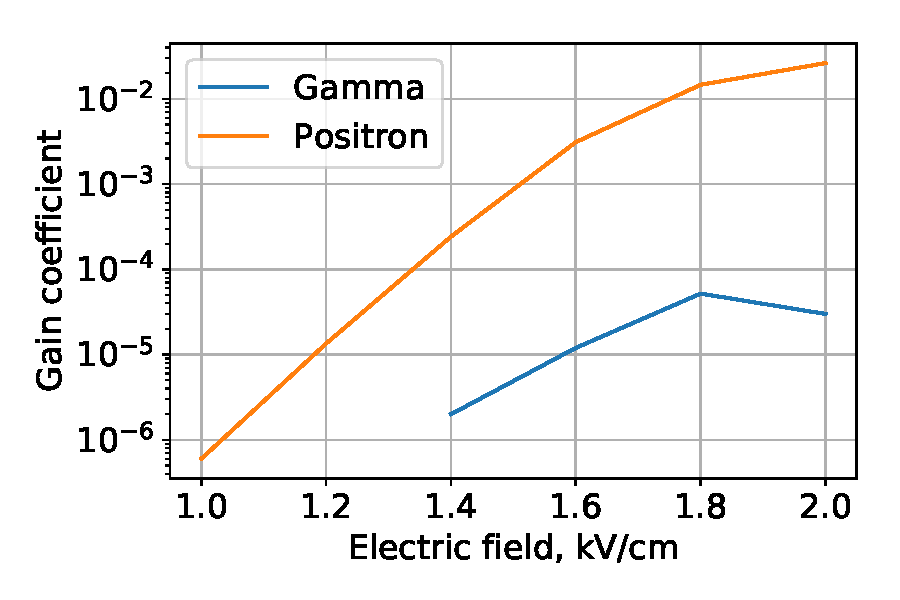
\includegraphics[width=0.5\linewidth]{pictures/08_gain}
        \label{pic-gain-a}
         \caption{Positron (gamma) feedback coefficient dependent on cell electric field for next parameters: primary electron energy - 3 MeV, field area size - 400 meter, electric field from 1 to 2 kV/cm, air density - $0.5 kg/m^3$ ($\sim 0.5 atm$)}
\end{center}
    	
   \end{figure}
         
% \begin{figure}[ht!]
% 	\begin{subfigure}[b]{0.5\textwidth}
%     	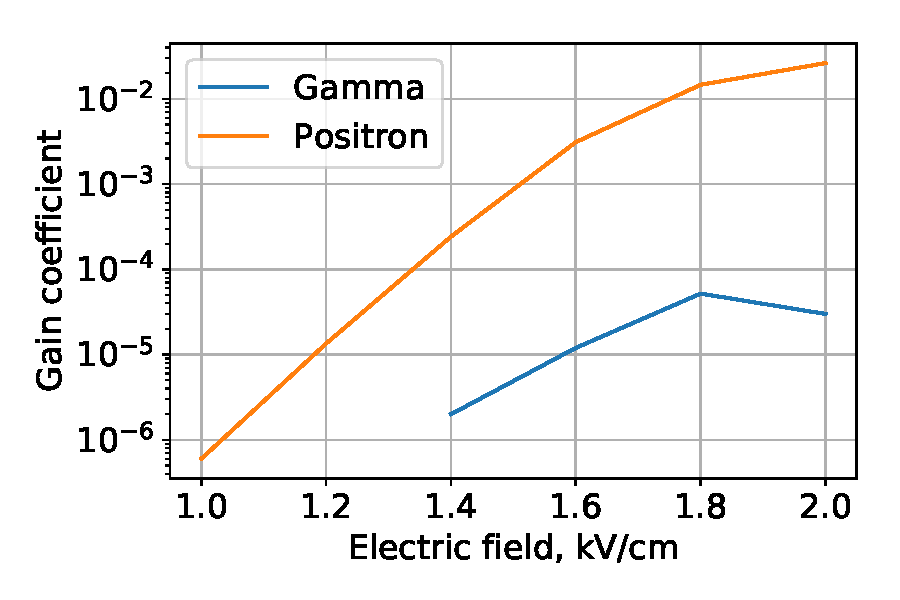
\includegraphics[width=0.95\linewidth]{pictures/08_gain}
%         \caption{}
%         \label{pic-gain-a}
%     \end{subfigure}
% 	~
%     \begin{subfigure}[b]{0.5\textwidth}
% 		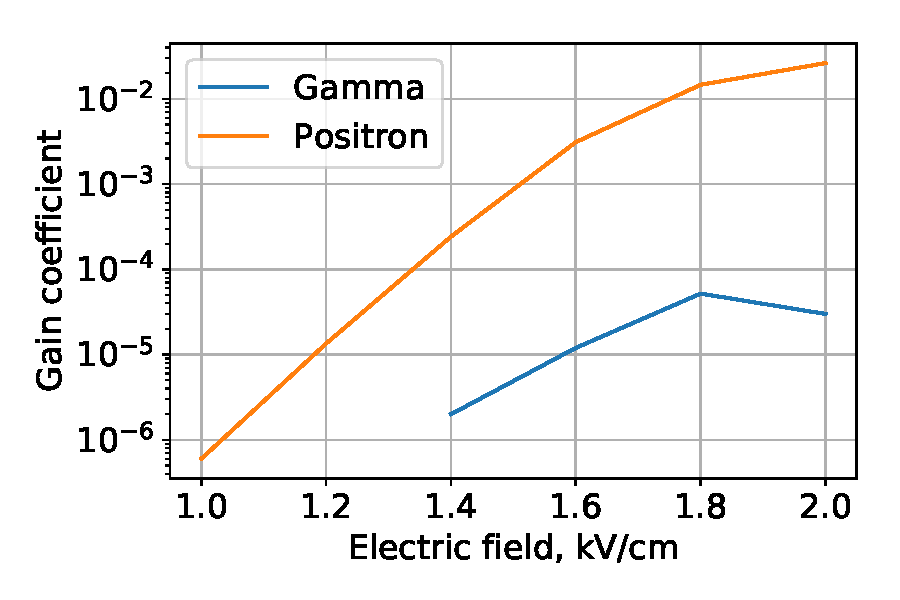
\includegraphics[width=0.95\textwidth]{pictures/08_gain}
%         \caption{}
%         \label{pic-dwayer-b}
%     \end{subfigure}
%     \caption{a) Positron (gamma) feedback coefficient dependent on cell electric field for next parameters: primary electron energy - 3 MeV, field area size - 400 meter, electric field from 1 to 2 kV/cm, air density - $0.5 kg/m^3$ ($\sim 0.5 atm$)
% %     b) Dwyer model in Geant 4 simulation. Red tracks – electrons. Blue tracks – positrons. Green tracks - gamma-rays
% }
% \end{figure}

\section{Discussion}
In this work, we get result, which different from Dwyer result. But by reason of high computing difficult Monte-Carlo simulation, we used several approximation, which inevitably influence on result precision. Although we leaded to choose approximation setting upper estimation of gain coefficient, this aim can't always be achieved. So for calculation of critical angle of reverse don't take to consideration elastic scattering, due to which several electron can turn at angles greater that critical angle. But analogy electron capable of reverse will be stopped by electric field, because we could take what procedure of selection by critical angle is right on average. Same exist necessary in increase of simulation statistics. Nevertheless getting estimation show what couldn't confidently affirm about strong influence positron (gamma) feedback mechanism on process in thunderstorm and. At the present time, we make precision Monte-Carlo simulation for getting final answer.

\section{Conclusion}
The paper presents a study of relativistic electron avalanches in cells with air density characteristic for atmosphere heights where clouds are formed and electric field value between 1 and 2.5 kV/cm. The result shows that positron gain coefficient in such cells is less than 0.01. Consequently, Dwyer feedback occurs rarely to increase runaway electron flux significantly.
The conditions when positron feedback coefficient is equal one were not determined. Nevertheless, Dwyer’s conditions~\cite{dwyer2003fundamental} were checked. In such conditions infinite electron avalanche reproduction works. However, the study shows that new electron avalanche models are needed to describe thunderstorm processes.

This work is supported by the Russian Science Foundation under grant No. 17-12-01439.
%This work is supported by the Ministry of Education and Science of the Russian Federation under the contract No. 3.3008.2017/PP.
   
\bibliography{references}{}
\end{document}
